%%%%%%%%%%%%%%%%%%%%%%%%%%%%%%%%%%%%%%%%%%%%%%%%%%%%%
%% Inserir seu texto da metodologia no campo abaixo %%
%%%%%%%%%%%%%%%%%%%%%%%%%%%%%%%%%%%%%%%%%%%%%%%%%%%%%
\chapter{Metodologia} 

\section{Tipo de Pesquisa}
O tipo de pesquisa escolhida foi quantitativa e exploratória, visando a viabilidade em se  desenvolver um aplicativo para busca de menor preço para uma compra com rota otimizada. O levantamento bibliográfico constitui-se de material já publicado de artigos científicos, livros, revistas e sites renomados da área.

\section{Método de Realização}
A opção pela pesquisa quantitativa tem por objetivo analisar o ponto de vista do público alvo do aplicativo proposto visando sua aceitação e viabilidade, podendo assim saber se uma aplicação de suporte a compras domésticas que tem por intuito oferecer a seus usuários onde encontrar o menor preço para suas compras levando em conta a melhor rota para tal é algo que a sociedade realmente precisa.

\section{Coleta de Dados}
Os dados foram levantados através de um formulário o qual foi disponibilizado de forma online para um grupo de 53 pessoas. Tais informações adquiridas com este foram essenciais para validar a viabilidade do projeto. 

Veja a seguir os dados levantados com tal formulário, no qual um grupo considerável de pessoas participaram:

Como esperado, mais de 75\% dessa população vai aos supermercados 2 a 10 vezes ao mês, conforme pode ser visto na figura \ref{fig:metodologia1}:

\begin{figure}[H]
    \centering
        \caption{Pergunta 01}
        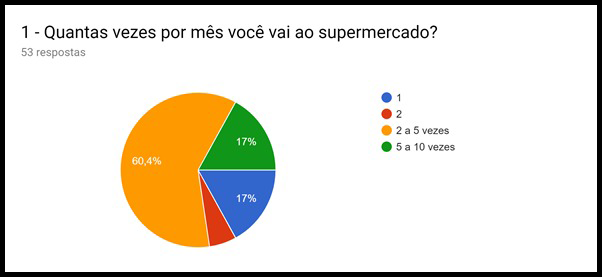
\includegraphics[scale=.8]{metodologia1.png}
        \label{fig:metodologia1}
		\fonte{Do autor - 2019}
\end{figure}


A maioria das pessoas sempre visita mais de um estabelecimento a fim de encontrar aquele que ofereça o melhor preço, conforme pode ser visto na figura \ref{fig:metodologia2} abaixo:

\begin{figure}[H]
    \centering
		\caption{Pergunta 02}
		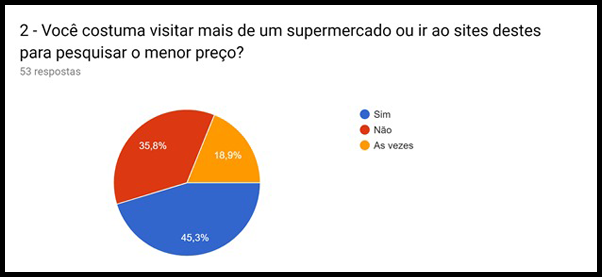
\includegraphics[scale=.8]{metodologia2.png}
		\label{fig:metodologia2}
		\fonte{Do autor - 2019}
\end{figure}

Nas visitas realizadas para a pesquisa de preço, há obviamente os gastos com transportes, seja de automóvel próprio ou transporte coletivo. A figura \ref{fig:metodologia3} traz esta informação.

\begin{figure}[H]
    \centering
		\caption{Pergunta 03}
		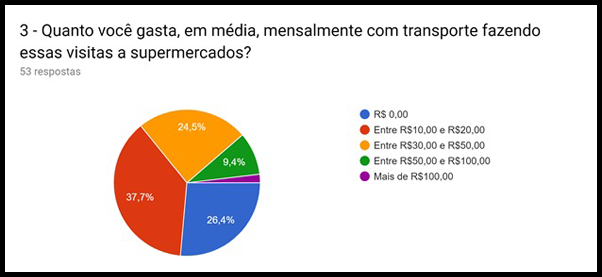
\includegraphics[scale=.8]{metodologia3.png}
		\label{fig:metodologia3}
		\fonte{Do autor - 2019}
\end{figure}

Há um gasto de tempo consideravelmente alto, levando em conta que para uma compra pessoas gastem tanto tempo visitando os supermercados. Demonstrado figura \ref{fig:metodologia4} abaixo.

\begin{figure}[H]
    \centering
		\caption{Pergunta 04}
		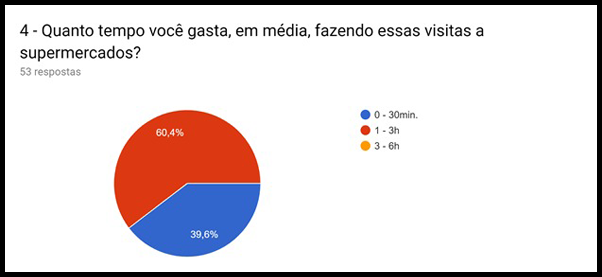
\includegraphics[scale=.8]{metodologia4.png}
		\label{fig:metodologia4}
		\fonte{Do autor - 2019}
\end{figure}

Indiscutivelmente, todas as pessoas entrevistadas usariam o aplicativo proposto. Conforme pode ser visto na figura \ref{fig:metodologia5}:
\begin{figure}[H]
    \centering
		\caption{Pergunta 05}
		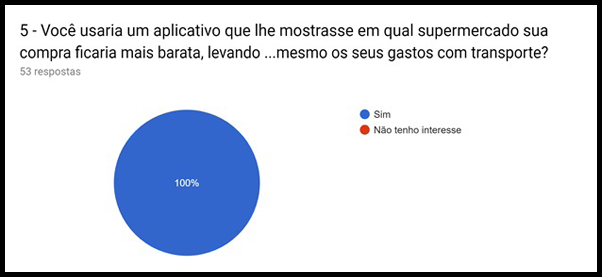
\includegraphics[scale=.8]{metodologia5.png}
		\label{fig:metodologia5}
		\fonte{Do autor - 2019}
\end{figure}

Pode se notar ainda que, quando se trata do tão escasso tempo, as pessoas estão dispostas a  abrirem mão da tão tradicional “experiência de compra”. O que pode ser visto na figura \ref{fig:metodologia6}.

\begin{figure}[H]
    \centering
		\caption{Pergunta 06}
		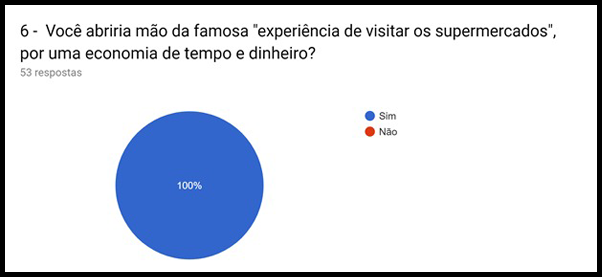
\includegraphics[scale=.8]{metodologia6.png}
		\label{fig:metodologia6}
		\fonte{Do autor - 2019}
\end{figure}

O formulário continha ainda questão aberta, visando analisar de forma mais dinâmica as opiniões dos supostos usuários: "... Um aplicativo que disponibiliza a seus usuários os menores preços para seus produtos, evitando que este, tenha gasto desnecessário de tempo e dinheiro fazendo pesquisas de preço..."
Na sua opinião, um supermercado aderiria um aplicativo com tal finalidade?

Foram obtidas diversas opiniões, as quais proporcionaram pontos de vista até então não trabalhados, porém prevaleceram as opiniões de pessoas que afirmaram ser totalmente necessário o uso do aplicativo na sociedade. Dentre as mais relevantes, pode se destacar:
“Sim, pois facilitaria imensamente a vida dos clientes dos supermercados, e os comércios devem adaptar-se aos clientes e não o contrário.”
“Sim, por saber que outros ramos do comércio já utilizam ferramentas do tipo para facilitar o alcance ao cliente. ”

Foi questionado também se as pessoas estariam dispostas a pagarem pelo uso do aplicativo, e pelo menos cerca de 1/3 destes se negaram a pagar, tal perspectiva reforça a hipótese de passar o custo diretamente para o estabelecimento ao invés de clientes ou cobrando 8\% encima de toda venda feita com o auxílio do aplicativo.

Um outro fato que ao ser inserido no aplicativo, e que poderia beneficiar tanto os estabelecimentos (divulgação de promoções) quanto clientes. Como é demonstrado na figura \ref{fig:metodologia9}.

\begin{figure}[H]
    \centering
		\caption{Pergunta 09}
		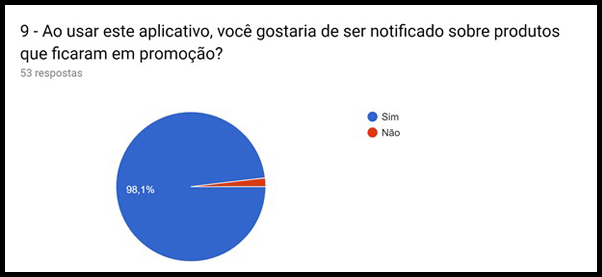
\includegraphics[scale=.8]{metodologia9.png}
		\label{fig:metodologia9}
		\fonte{Do autor - 2019}
\end{figure}

% \section{Critérios de Delimitação}
% Digite seu texto nesse campo.

% \section{Instrumentos de Pesquisa}
% Digite seu texto nesse campo.

% \section{Tratamento dos Dados}
% Digite seu texto nesse campo.